This chapter will discuss the process of implementing the application. The justification of the technologies used along with the benefits, and, challenges they potentially presented will be discussed here.

\section{Version Control}
Version control is required to have been used throughout the duration of the project. Version control allows us to keep track and manage changes made to source code and other software artefacts. Good utilization of version control is critical to the success of a project, and helps to keep a project organised.
\subsection{GitHub \& Git}
GitHub \cite{github} is a platform widely used throughout the industry to store software projects online. GitHub allows users to create Git repositories \cite{git} that contain the files used within a project along with their version history. This combination is widely used within the industry due to the distributed version control and the various tools offered by GitHub to enhance the developer experience. Both these tools were very familiar so made this a simple choice. 
\subsubsection{Feature Branching}
An advantage of using a distributed version control system such as Git is how easy branching is due to the developer being able to create multiple branches at a local level. Feature branching was used throughout this project (see \ref{fig:branching}), with new features being developed in local feature branches and then merged back with the main branch upon completion.  
\begin{figure}[!htbp]
    \centering
    \begin{subfigure}[b]{0.90\textwidth}
        \frame{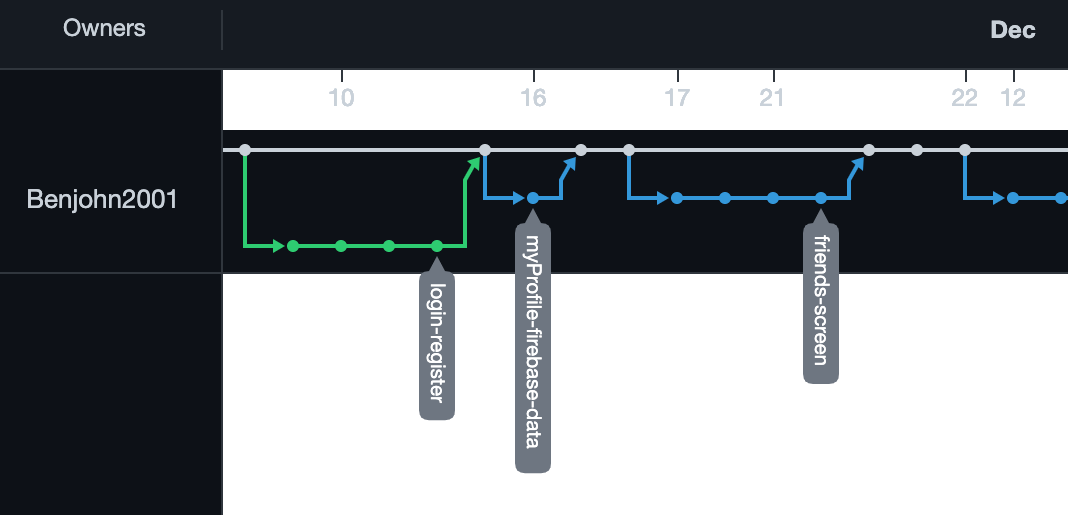
\includegraphics[width=\textwidth]{featureBranch.png}}
    \end{subfigure}
    \caption{Example of feature branching used in project}
    \label{fig:branching}
\end{figure}
\subsubsection{Issue Tracking}
The GitHub issue tracker was used to keep track of what tasks were still to be completed, along with any bugs that needed to be fixed. GitHub allows you to apply labels to an issue helping you to separate between Firebase and design issues for example (see \ref{fig:issues}).
\begin{figure}[!htbp]
    \centering
    \begin{subfigure}[b]{0.90\textwidth}
        \frame{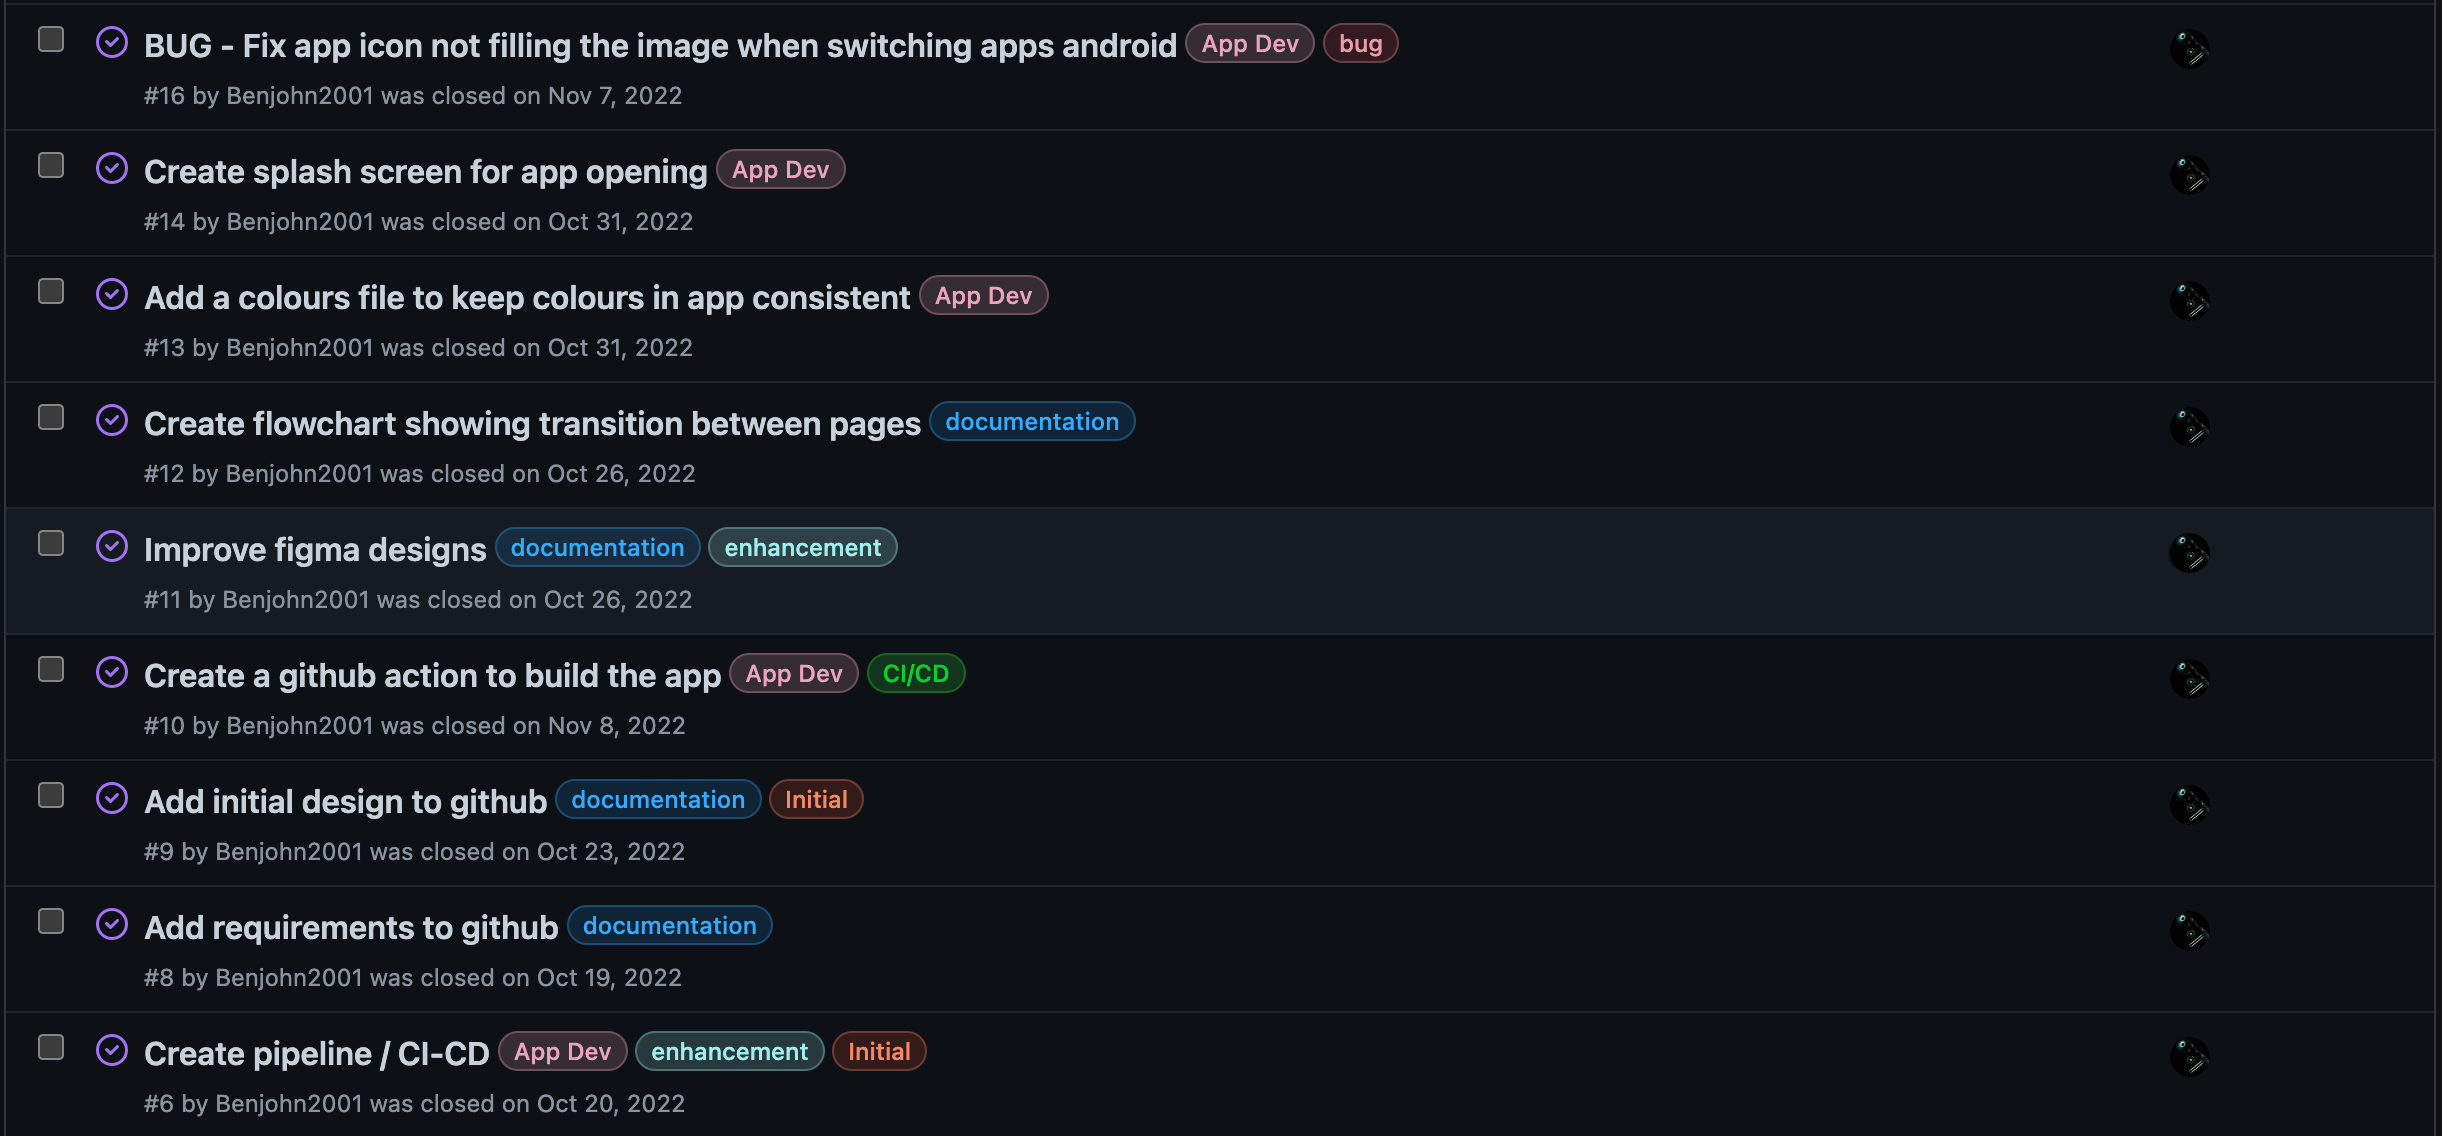
\includegraphics[width=\textwidth]{issues.png}}
    \end{subfigure}
    \caption{Examples of issues created in GitHub's issue tracker}
    \label{fig:issues}
\end{figure}
\subsubsection{Actions}
GitHub's actions is a continuous integration and continuous delivery tool that allows you to create workflows that are triggered on specific behaviour. A workflow that built and published the application upon a push to the main branch was created so that the newest version of the app was always accessible on my mobile device. A testing workflow was also created with any pushes to the tests, or main branch running the test suite along with code formatting and style checks (see \ref{CodeF&S}).
\section{Technologies}
A comparative study \cite{compStudy} was performed in the early stages to help decide what technologies were best suited to the task. The technologies used throughout the project will be discussed in this section.
\subsection{React Native}
When creating a mobile application you currently have two options, native applications for each operating system, or, using frameworks that allow a single code base to create applications for both operating systems. While there are many positives from creating native apps such as being able to utilize many platform specific features, the extra development time to create two consistent, but separate apps was simply infeasible within the time constraints. React Native \cite{reactnative} allows you to create whole applications using only JavaScript \cite{js} in a singular code base. This was chosen over other alternative due to the component nature and flexibility provided by the framework. 
\subsubsection{Expo}
Solely React Native development does however require some native coding and the presence of build tools for both operating systems which was an issue. This meant that both Android Studio and XCode would both have to be installed on the device used for developing the application which was an issue for storage space. Due to no native coding being required in the project the choice to use Expo \cite{expo}, a framework used to help ease building React Native applications was made. Expo requires no native coding or build tools allowing you to simply run a command in the terminal to be able to access the application on your device or emulator.
\begin{figure}[!htbp]
\centering
\begin{subfigure}[b]{0.5\textwidth}
\begin{lstlisting}[language=bash]
  $ expo start --ios
  $ expo start --android
\end{lstlisting}
\end{subfigure}
\caption{To build and start applications with expo for iOS or Android}
\end{figure}
\subsection{Tailwind CSS}
When creating a user interface there are several CSS frameworks and UI kits that can be used in tandem, or, independently of standard CSS style sheets. Tailwind CSS \cite{tailwind} is a CSS framework that allows the developer to create reusable styled components simply by using utility classes in the className property. Tailwind does not include styled components giving full control to the developer over the design. This approach was chosen over a UI kit of created components to allow the design to be unique and flexible to the project requirements. NativeWind \cite{nativewind} is a package used to process the CSS from the tailwind class names into StyleSheet objects, that can then be understood by ReactNative. The use of this technology enhanced the user interface and developer experience by allowing full flexibility over design, and, an easier alternative to traditional CSS style sheets. 
\begin{figure}[!htbp]
    \centering
    \begin{subfigure}[b]{0.42\textwidth}
        \begin{lstlisting}[language=jsJsx, caption={Styled using Tailwind CSS}]
        <TouchableOpacity
            onPress={onPressFunction}
            className="bg-darkerPurple h-12 w-10/12 rounded-full"
        >
            <Text className="text-white text-center">
                Press Me
            </Text>
        </TouchableOpacity>
        \end{lstlisting}
    \end{subfigure}
    \hspace{2em}
    \begin{subfigure}[b]{0.45\textwidth}
        \begin{lstlisting}[language=jsJsx, caption={Styled using a traditional StyleSheet}]
        <TouchableOpacity
            onPress={onPressFunction}
            style={styles.button}
        >
            <Text style={styles.text}>
                Press Me
            </Text>
        </TouchableOpacity>
            
        const styles = StyleSheet.create({
          button: {
            justifyContent: 'center',
            backgroundColor: 'purple',
            borderRadius: 9999,
            height:48,
            width:200,
          },
          text: {
            textAlign: 'center',
            color: 'white'
          },
        });
        \end{lstlisting}
    \end{subfigure}
    \caption{Example of a simple styled button}
    \label{fig:tailwind}
\end{figure}
\FloatBarrier
\subsection{Code Formatting \& Style} \label{CodeF&S}
To ensure the code base was consistent, and free of bugs the code formatter Prettier \cite{prettier}, and, code analysis tool ESLint \cite{eslint} were used. Prettier rewrites code into a consistent style, this ensures that all files throughout the project are consistent. ESLint is a linter used with JavaScript to analyze code finding errors and enforcing a chosen code style. Airbnb \cite{airbnb} code style was chosen for this project as this is the most popular JavaScript style guide. Both these tools were used together to ensure bug free, consistent and readable code. 
\subsection{Firebase}\label{firebaseSection}
To store and authenticate the data for the application Google's Firebase \cite{firebase} platform was chosen. Firebase allows developers to have real-time access to hosted services from the client-side code. Firebase was chosen due to being optimised for mobile applications with real-time NoSQL \cite{nosql} databases, and, many other helpful services. Although Firebase has a paid tier the free tier would suffice for this project.     
\subsubsection{Authentication}
Firebase provides an authentication service to allow the application to verify the identity of a user. The service is easy to set-up and use throughout other services, and, very secure due to being maintained and developed by Google.
\subsubsection{Storage}
Firebase cloud storage was used to store all the images used throughout the application. This was easy to implement with references to these images being stored in the database, and the images themselves securely uploaded and downloaded from the cloud storage.
\subsubsection{Realtime Database}
The application data is stored in a NoSQL, cloud hosted  database through Firebase's realtime database service. This allows for real-time syncing of data keeping the application up to date with any changes made. This requires no servers and is relatively easy to set-up, manage, and, scale.
\begin{figure}[!htbp]
\centering
\begin{subfigure}[b]{0.85\textwidth}
\begin{lstlisting}[language=json]
"KKSw9RsMRlSBKjUy7EGOiA1NcFk2": {
    "bio": "Im ben who shops at iceland",
    "email": "benjohnston2001@icloud.com",
    "firstName": "Ben",
    "lastName": "Johnston",
    "profilePic": "images/profilePics/KKSw9RsMRlSBKjUy7EGOiA1NcFk2",
    "userName": "Benjohn2001"
  },
\end{lstlisting}
\end{subfigure}
\caption{How data is stored in the Realtime Database as JSON objects.}
\small\par\textit{{The key "KKSw9RsMRlSBKjUy7EGOiA1NcFk2", used to access this object in the database, and the user data, including the path to the users profile picture in cloud storage.}}
\label{jsonResp}
\end{figure}

\section{Final Product}
The final product produced provides the user with an easy to use, and elegant application that encompasses all of the must, and, should have requirements. The application uses a consistent design throughout paired with an intuitive navigation system to make the  application easy to learn and use. Users can register for an account, add their friends, then create groups which they can use to track their friends status on a graphical clock.
\subsection{User Interface}
By exploiting react natives component based architecture, reusable UI components were constructed and used throughout the application to streamline the implementation, while keeping the design consistent (see \ref{appendix:appScreens}).
\subsubsection{WCAG}
The web content accessibility guidelines \cite{wcag}, are a set of accessibility guidelines created by the World Wide Web Consortium (W3C) \cite{w3c} outlining how to make web content more accessible for users with disabilities and impairments. These guidelines also apply to mobile applications and are recommended by the UK government \cite{govWCAG} to help developers create more accessible mobile apps. Some examples of where effort was made to conform to these guidelines are detailed below.
\begin{figure}[!htbp]
    \centering
    \begin{subfigure}[b]{0.45\textwidth}
        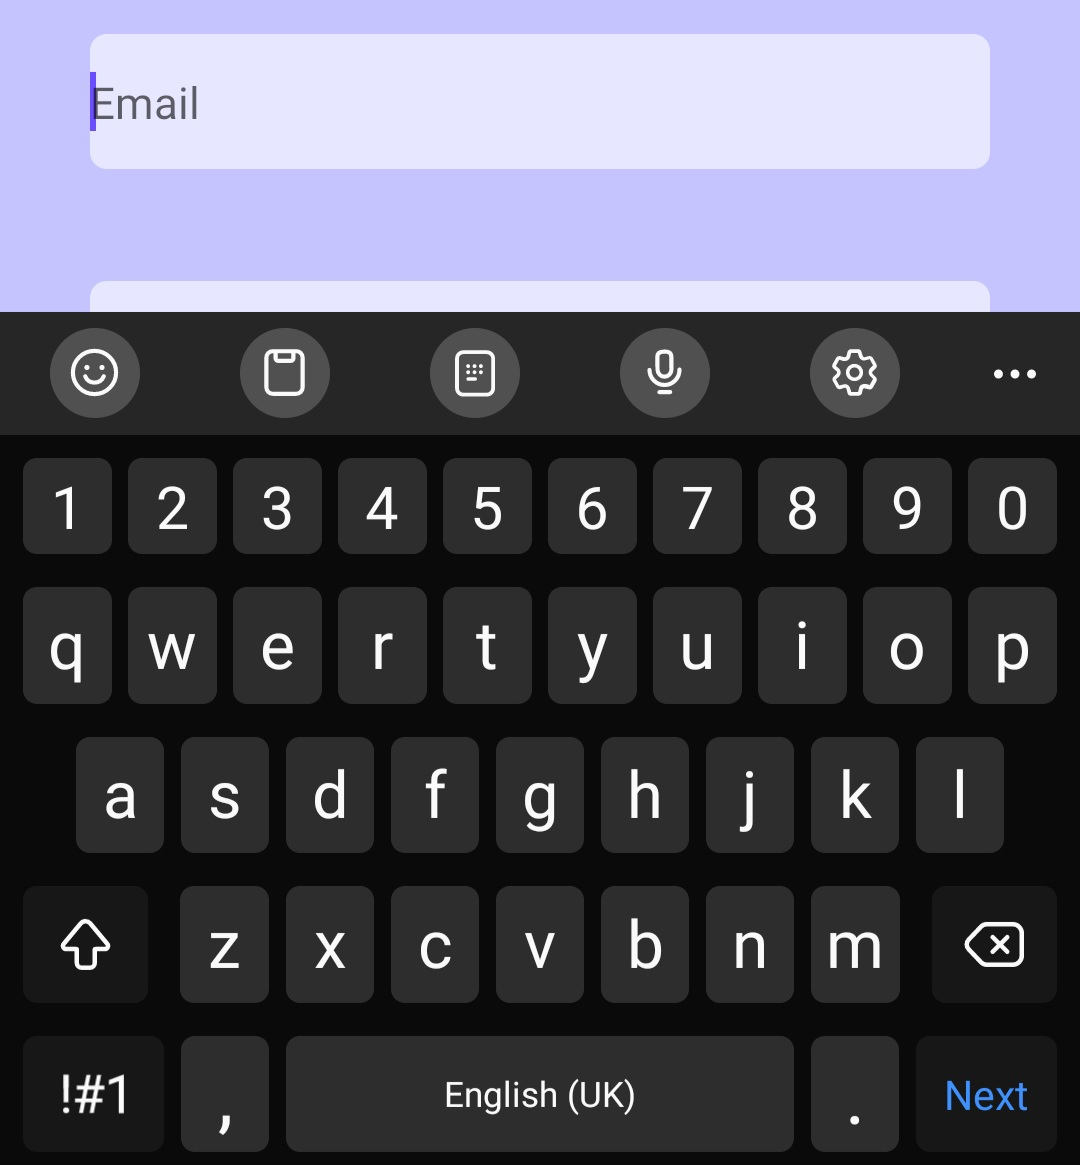
\includegraphics[width=\textwidth, height=5.5cm]{keyboard.jpg}
        \caption{\textbf{Keyboard \& Text Input:} The keyboard shifts focus to the text input box when selected and allows navigation of the form through overriding the return key to 'Next, and, 'Done' \textbf{(Success Criterion 3.2.2)}. A cursor also highlights the current text box selected.}
    \end{subfigure}
    \hspace{1.5em}
    \begin{subfigure}[b]{0.45\textwidth}
        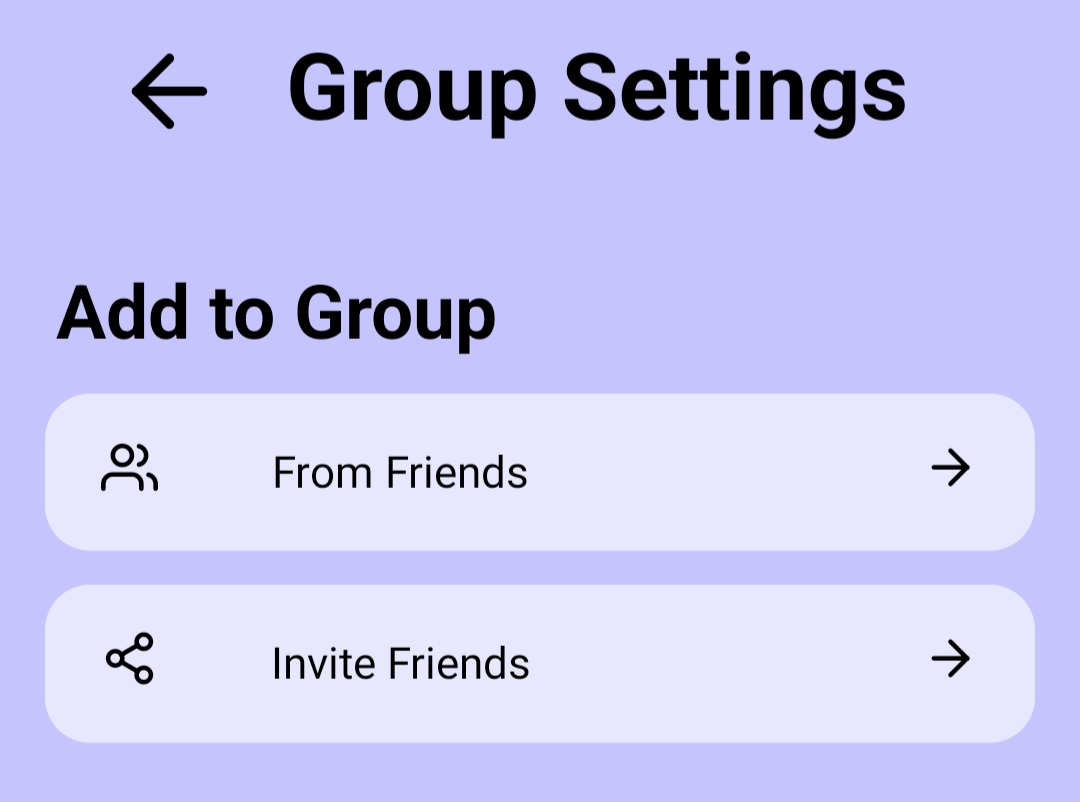
\includegraphics[width=\textwidth]{navigable.jpg}
        \caption{\textbf{Navigable:} Application screens have clear and consistent titles and navigation options helping users navigate, and, determine their location. Headings are used to separate UI components which make the use of icons to help guide the user \textbf{(Success Criterion 2.4.2 \& 2.4.6)}.  }
    \end{subfigure}
    \vskip\baselineskip
    \begin{subfigure}[b]{0.45\textwidth}
        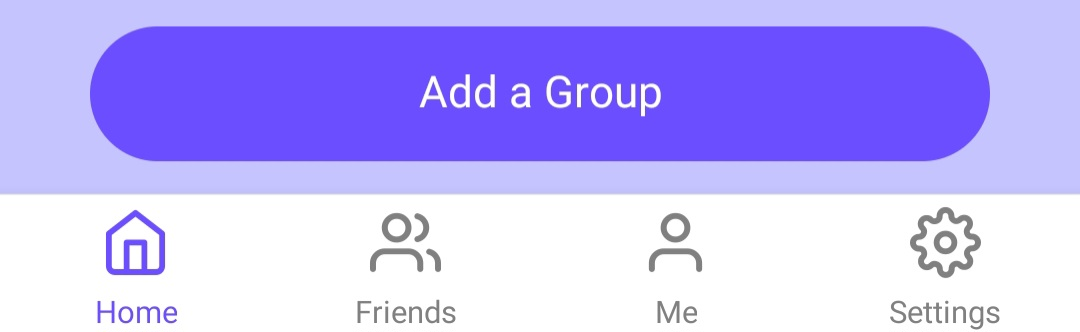
\includegraphics[width=\textwidth]{navbar.jpg}
        \caption{\textbf{Location:} Current location is displayed within the navigation bar \textbf{Success Criterion 2.4.8} }
    \end{subfigure}
    \caption{Examples of accessibility conformance throughout application}
    \label{fig:accesibility}
\end{figure}
\FloatBarrier
\subsubsection{UI Implementation}


\subsection{Back End of Application}
As discussed in \ref{firebaseSection}, Firebase was used to store and manage all the data for the application, including graphics, and, authentication data. Firebase realtime database is a NoSQL database architecture storing data as objects in a JSON tree, as shown in figure \ref{jsonResp}. Application data was stored in the JSON objects users(user data), clockFace(clock background), friends(a users friends list), groupMembers(a groups members), groups(a users groups), and, locations(storing a groups locations) (see \ref{appendix:rtdb}). As we are unable to store images in the realtime database image paths were stored, and then used to download the image when needed from cloud storage. User images were stored by user id allowing easy updates due to old images being overwritten and, not stored. An email and password were used to create accounts and be authenticated. Firebase authentication provided easy to use SDKs facilitating sign in, forgotten password, and, the registering of new users. The sole use of Firebase throughout this project allowed the back end of the application to stay centralized within a sole platform, making it easier to implement and maintain. A diagram visualising the use of these Firebase services is shown below (see \ref{fig:firebaseDiag}).
\begin{figure}[!htbp]
    \centering
    \begin{subfigure}[b]{\textwidth}
        \frame{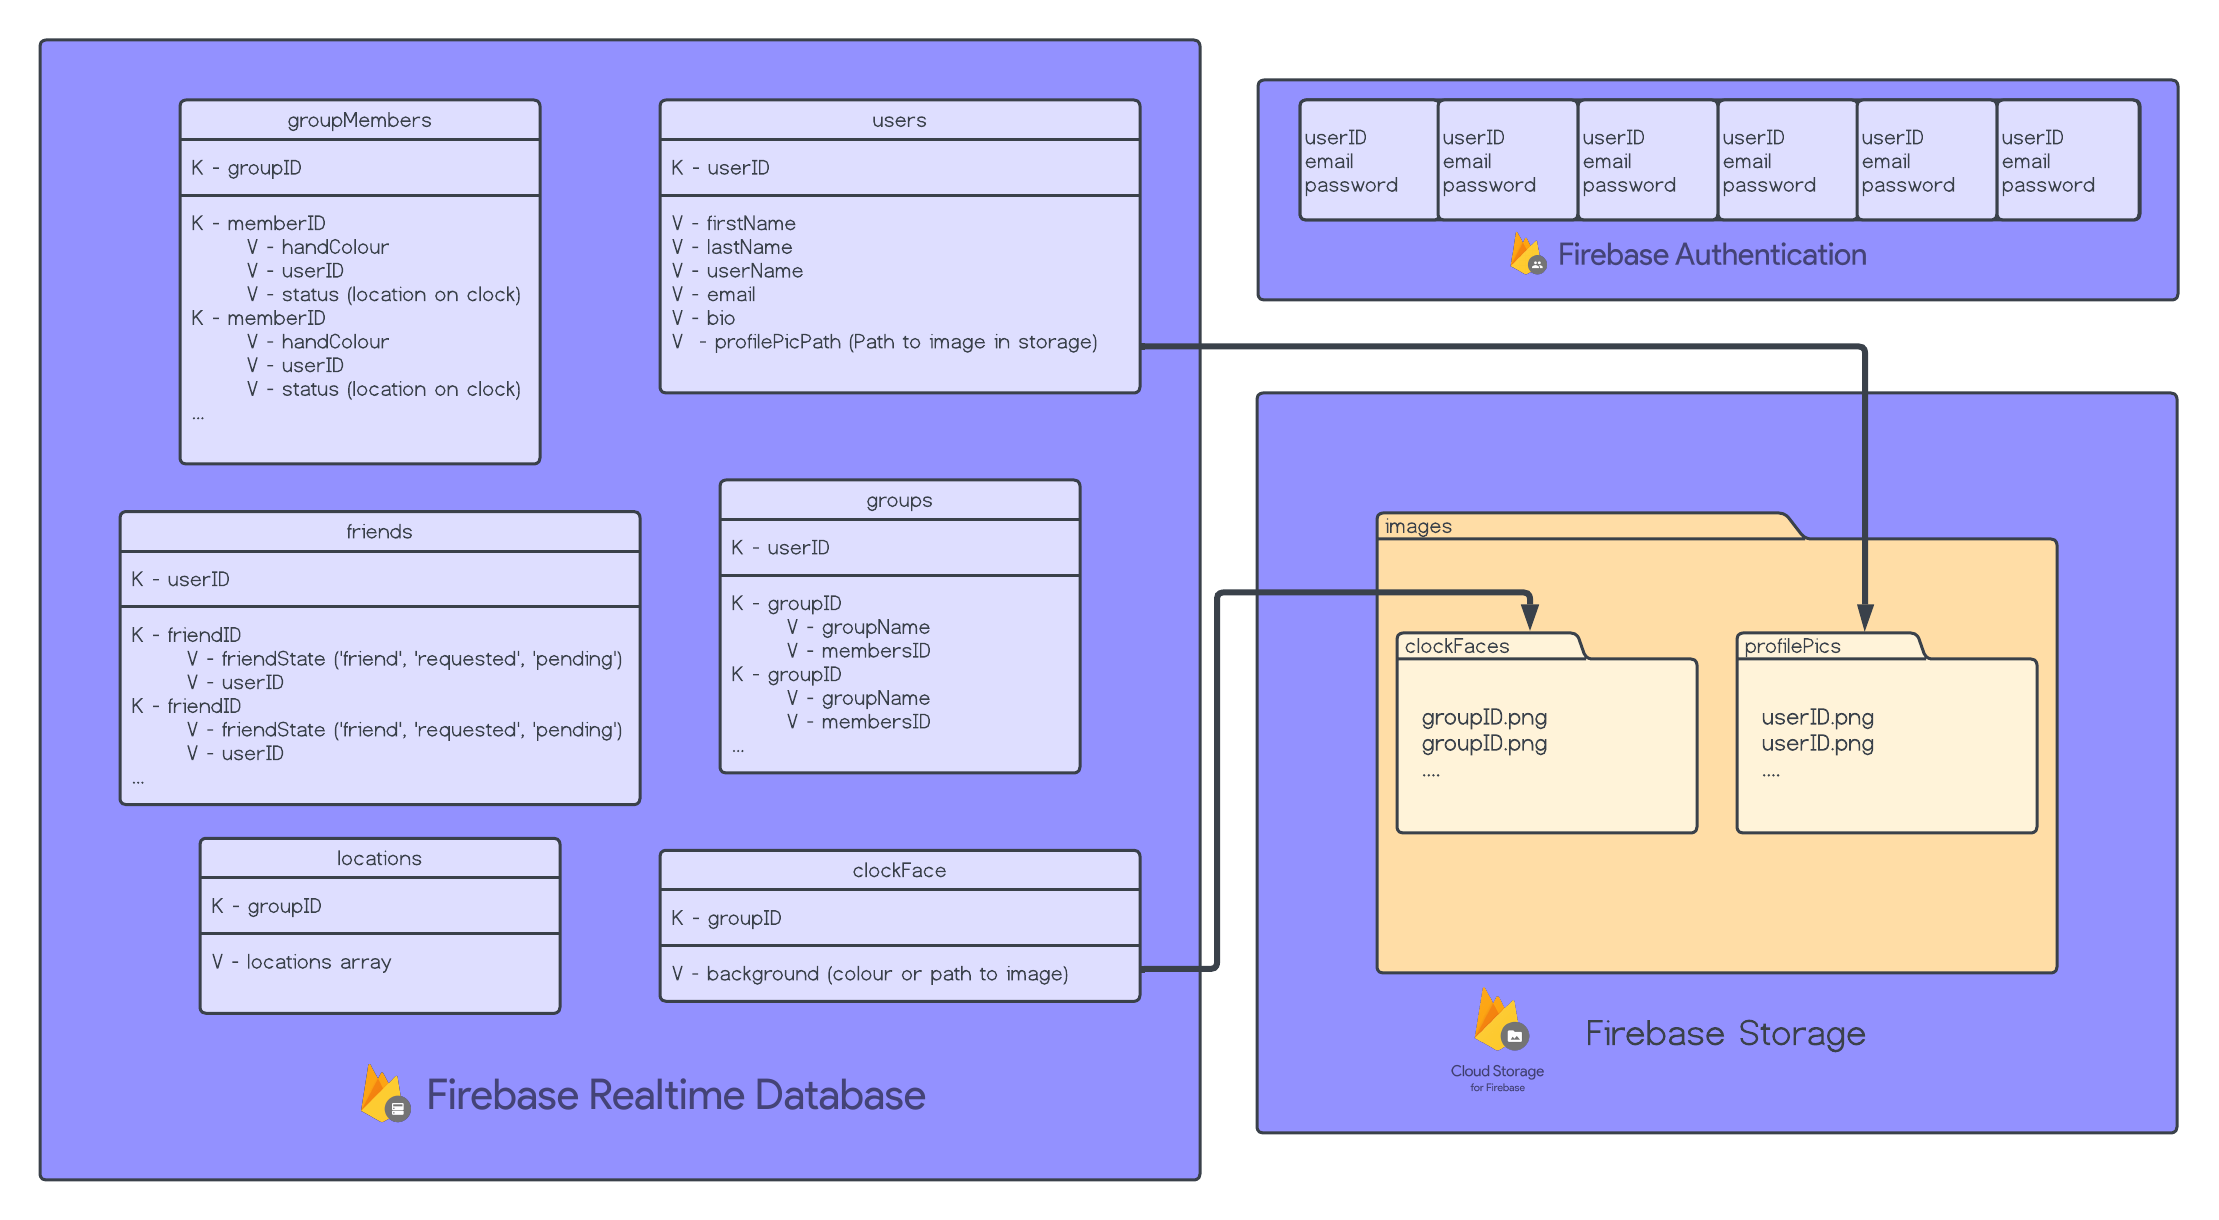
\includegraphics[width=\textwidth]{firebaseDiag.png}}
    \end{subfigure}
    \caption{Diagram visualising how data is stored in Firebase} \small\textit{{Logos: \cite{storImg, rtdbImg, authImg}}}
    \label{fig:firebaseDiag}
\end{figure}
\FloatBarrier
\section{Challenges}
